\documentclass{article}
\usepackage{tikz}
\usepackage{amsmath}
\usetikzlibrary{datavisualization}
\title{CSL 603 - Machine Learning\\Lab 1\\Decision Trees and Forests}
\author{Aditya Gupta\\2015csb1003}
\begin{document}
\maketitle
\section*{Decision Tree (Experiment 2)}
A decision tree was learnt using 1000 reviews from the train set and tested on 1000 reviews from the test set. The learned tree showed the following statistics:
\subsection{Effect of Early Stopping}
The tree propagation was stopped when a critical height was reached and various properties of the tree such as total terminal nodes (leaf nodes) and the accuracy was noted. The following results were obtained:
\begin{itemize} 
\item Increase in Training Accuracy as maximum height increased as tree more and more fitted to the training data. The Testing accuracy initially increased but then became almost constant and then slightly decreased due to overfitting.

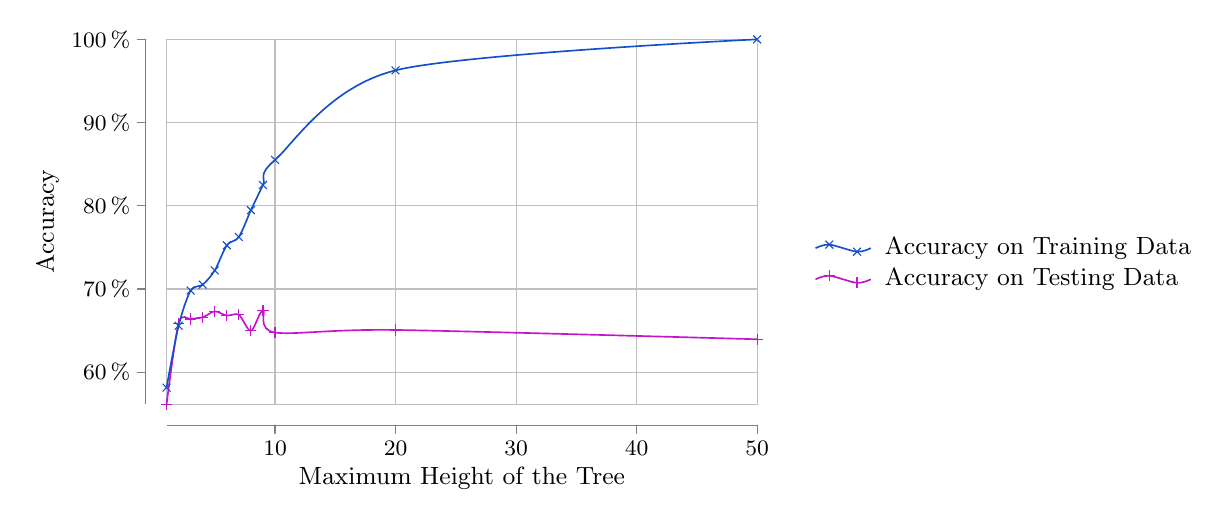
\begin{tikzpicture}[scale=1.5]
\datavisualization [scientific axes=clean,
	x axis={grid, label={Maximum Height of the Tree}},
	y axis={grid, label={Accuracy}, ticks ={tick unit=\%}},
	visualize as smooth line/.list={trainacc, testacc},
	style sheet=vary hue,
	style sheet=cross marks,
	trainacc={label in legend={text=Accuracy on Training Data}},
	testacc={label in legend={text=Accuracy on Testing Data}}]
data [set=trainacc] {
	x, y
	1, 58.148
	2,65.593
	3,69.818
	4,70.523
	5,72.233
	6,75.251
	7,76.257
	8,79.476
	9,82.494
	10,85.513
	20,96.277
	50,100.000
}
data [set=testacc] {
	x, y
	1,56.142
	2,65.888
	3,66.395
	4,66.598
	5,67.309
	6,66.802
	7,66.903
	8,64.974
	9,67.411
	10,64.771
	20,65.076
	50,63.959
};
\end{tikzpicture}

\item The total number of leaf nodes increased slowly as height increased as more and more splits occured and thus resulting in more leaf nodes.

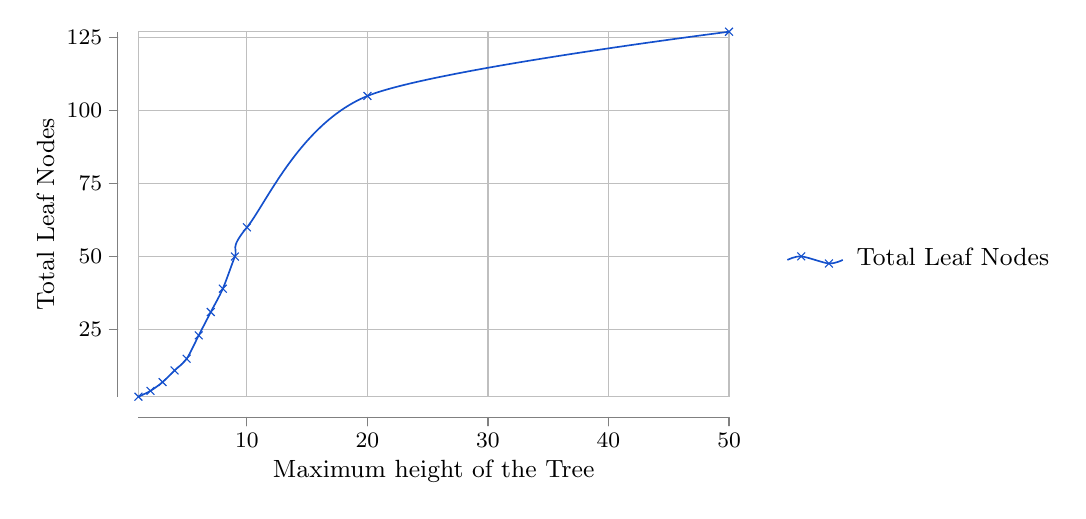
\begin{tikzpicture}[scale=1.5]
\datavisualization [scientific axes=clean,
	visualize as smooth line/.list={leaf},
	style sheet=vary hue,
	style sheet=cross marks,
	x axis={grid, label={Maximum height of the Tree}},
	y axis={grid, label={Total Leaf Nodes}},
	leaf={label in legend={text=Total Leaf Nodes}}]
data [set=leaf]{
x, y
1,2
2,4
3,7
4,11
5,15
6, 23
7, 31
8, 39
9, 50
10, 60
20, 105
50, 127
};
\end{tikzpicture}

\item Some of the commonly used words to decide were ``this'', ``where'', ``town'', ``moments'' and ``he''.

\end{itemize}

\section*{Noise (Experiment 3)}
The Noise was changed and the following results were obtained:

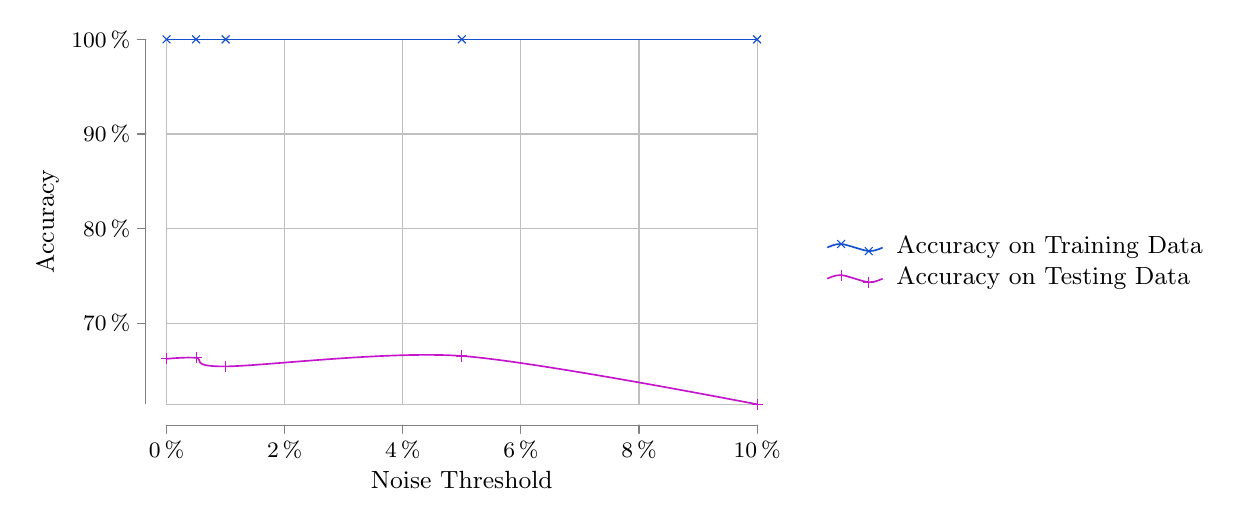
\begin{tikzpicture}[scale=1.5]
\datavisualization [scientific axes=clean,
	x axis={grid, label={Noise Threshold}, ticks={tick unit=\%}},
	y axis={grid, label={Accuracy}, ticks ={tick unit=\%}},
	visualize as smooth line/.list={trainacc, testacc},
	style sheet=vary hue,
	style sheet=cross marks,
	trainacc={label in legend={text=Accuracy on Training Data}},
	testacc={label in legend={text=Accuracy on Testing Data}}]
data [set=trainacc] {
	x, y
	0, 100.0
	0.5, 100.0
	1, 100.0
	5, 100.0
	10, 100.0
}
data [set=testacc] {
	x, y
	0, 66.232
	0.5, 66.332
	1, 65.430
	5, 66.533
	10, 61.422
};
\end{tikzpicture}

\section*{Pruning (Experiment 4)}
Lorem Ipsum bla bla bla

\section*{Decision Forests (Experiment 5)}
A decision forest was constructed using $5, 10, ... 50$ trees  with $\sqrt{N}$ where $N$ are the attributes occuring in the $1000$ trees and the following results were obtained:

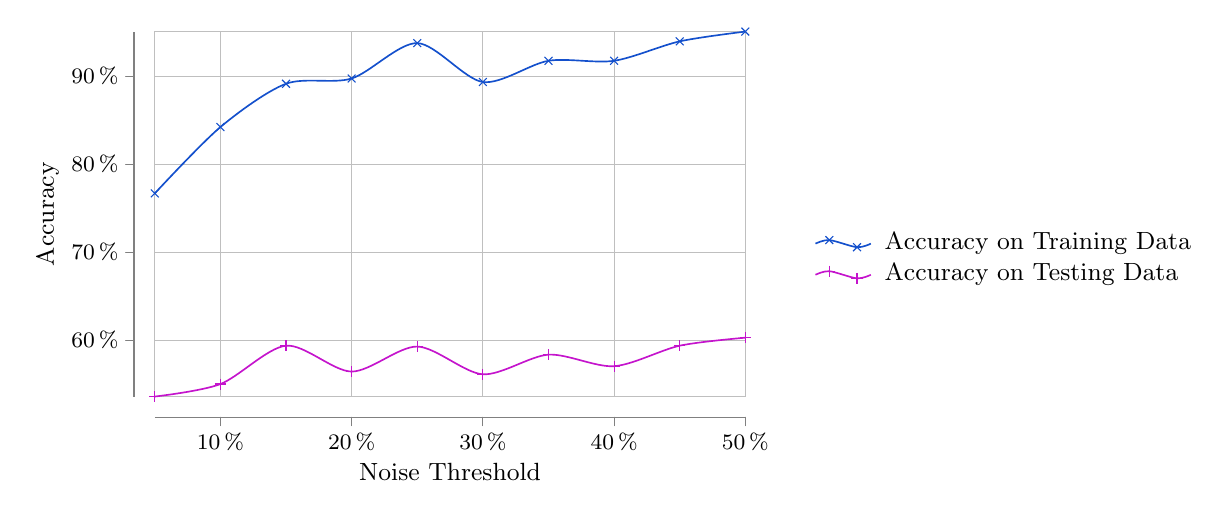
\begin{tikzpicture}[scale=1.5]
\datavisualization [scientific axes=clean,
	x axis={grid, label={Noise Threshold}, ticks={tick unit=\%}},
	y axis={grid, label={Accuracy}, ticks ={tick unit=\%}},
	visualize as smooth line/.list={trainacc, testacc},
	style sheet=vary hue,
	style sheet=cross marks,
	trainacc={label in legend={text=Accuracy on Training Data}},
	testacc={label in legend={text=Accuracy on Testing Data}}]
data [set=trainacc] {
	x, y
	5, 76.68
	10, 84.22
	15, 89.14
	20, 89.74
	25, 93.76
	30, 89.34
	35, 91.75
	40, 91.75
	45, 93.96
	50, 95.07
}
data [set=testacc] {
	x, y
	5, 53.59
	10, 55.01
	15, 59.37
	20, 56.43
	25, 59.27
	30, 56.12
	35, 58.35
	40, 57.04
	45, 59.37
	50, 60.28
};
\end{tikzpicture}
\end{document}